\section{模型检验与分析}
\label{sec:validation}

本文构建物理可行性、信息集 mutation、计划持续性、结算分解和历史配置回归五类自动验证，最终主结果全部通过。

\subsection{物理可行性与数值精度}

对问题一、问题二四组对照、问题三主消融与配对控制、结算敏感性以及问题四全部年度方案逐时回代，检验母线平衡、SOC 递推、边界、互斥和费用分解，结果见表~\ref{tab:validation}。

\begin{table}[htbp]
	\caption{模型检验结果汇总}
	\label{tab:validation}
	\centering
	\zihao{-5}
	\begin{tabular}{l l l l}
		\toprule
		检验项目 & 最大值 & 验收阈值 & 结论 \\
		\midrule
		母线能量平衡残差 & $<10^{-12}$ kWh & $10^{-7}$ kWh & 通过 \\
		储电量递推残差 & $<10^{-12}$ kWh & $10^{-7}$ kWh & 通过 \\
		储电量取值区间 & $[1200,\ 10800]$ kWh & 同上 & 通过 \\
		主方案同时充放电量 & $<10^{-8}$ kWh & $10^{-5}$ kWh & 通过 \\
		问题三费用分解回代差 & $<10^{-8}$ 元 & $10^{-7}$ 元 & 通过 \\
		Excel 回读与逐时明细差异 & $<10^{-10}$ & 数值一致 & 通过 \\
		\bottomrule
	\end{tabular}
\end{table}

连续模型由词典序目标排除无效吞吐，叠加结算主模型由式~\eqref{eq:mutual-exclusive} 严格禁止同时充放电。问题三总费用与“计划费 $+$ 调整费 $+$ 紧急费”直接回代一致。五个结果工作簿保留附件 5 的工作表结构与格式，回读数值与逐时明细一致。

\subsection{未来信息泄漏的 mutation 测试}

物理约束只能保证结果可行，不能保证结果\emph{可实现}。为此本文设计了四组因果性篡改实验与一组计划持续性检验，直接检查信息集因果性：

\begin{enumerate}[label=(\arabic*), itemsep=2pt, topsep=2pt]
	\item \textbf{问题二负载因果性}：把第 $d$ 天真实负载整体乘以 $10$，在不改动 $d$ 日之前历史数据的条件下重新求解，要求第 $d$ 天 $0{:}00$ 的计划输入完全不变（最大偏差 $<10^{-10}$）；
	\item \textbf{问题二光伏因果性}：同法篡改第 $d$ 天真实光伏，要求 $0{:}00$ 的光伏计划输入完全不变；
	\item \textbf{问题三节点因果性}：篡改第 $d$ 天 $6{:}00$ 之后的真实负载与真实光伏，要求 $6{:}00$ 决策输入与结果不变；后续节点可合法使用已经执行完的观测；
	\item \textbf{问题四价格因果性}：篡改第 $d$ 天 $6{:}00$ 之后的附件 4 真实电价，要求因果价格模式下 $6{:}00$ 决策不变，而附件 4 直用模式下应当改变。
	\item \textbf{计划持续性}：仅启用 $0{:}00,6{:}00$ 时，核对后续切片均来自 $6{:}00$ 更新的有效计划，而非回退到 $0{:}00$ 基准计划。
\end{enumerate}

五组测试全部通过。第 (4) 组中同一篡改确实会改变附件 4 直用结果，说明因果扩展下的“不变”来自信息隔离而非篡改无效；第 (5) 组直接覆盖了节点消融最容易出现的计划回退错误。

\subsection{结算口径的单元测试}

按题目文字直接手算校验两种口径的费用公式。取 $\pi=1$ 元/kWh：

\begin{itemize}[itemsep=1pt, topsep=2pt]
	\item replacement：$G^{p}=900,\,G^{a}=700\Rightarrow 700+0.5\times200=800$；$G^{p}=700,\,G^{a}=900\Rightarrow 700+1.5\times200=1000$；
	\item additive：$G^{p}=900,\,G^{a}=700\Rightarrow 900+0.5\times200=1000$；$G^{p}=700,\,G^{a}=900\Rightarrow 700+1.5\times200=1000$。
\end{itemize}

两组手算结果与程序输出一致。在随机负载／光伏／价格序列上，优化目标与直接回代公式之差小于 $10^{-7}$；两种口径分别重优后，各自费用均不高于把另一口径方案直接代入所得的费用。

\subsubsection{充放电互斥的混合整数检验}

连续松弛在叠加结算下可能利用“边充边放”耗散 SOC；本文在主模型的每个 $24$ h 滚动窗口中设置至多 $144$ 个二元变量 $z_t$，由式~\eqref{eq:mutual-exclusive} 保证充放电互斥。全年主方案最大同时充放电量低于 $10^{-8}$ kWh，所有滚动子问题均达到最优状态，说明互斥约束已排除该退化现象。

\subsection{历史配置的回归复现}

为确认修订没有破坏原有工程，本文在旧参数组合（完美负载、附件 4 直用、实时反馈、非对称风险边际、差额结算、日循环终端且不用典型日先验）下重新运行四问，与既有结果逐项比对：

\begin{table}[htbp]
	\caption{历史配置结果回归比对}
	\label{tab:regression}
	\centering
	\zihao{-5}
	\begin{tabular}{l r r r}
		\toprule
		结果 & 修订前/元 & 修订后/元 & 绝对偏差/元 \\
		\midrule
		问题一 & 35\,126.9486 & 35\,126.9486 & $<10^{-3}$ \\
		问题二 & 13\,276\,966.0012 & 13\,276\,966.0012 & $<10^{-3}$ \\
		问题三 & 13\,048\,124.9508 & 13\,048\,124.9508 & $<10^{-3}$ \\
		问题四-2 & 13\,949\,811.6640 & 13\,949\,811.6640 & $<10^{-3}$ \\
		问题四-3 & 13\,734\,900.0034 & 13\,734\,900.0034 & $<10^{-3}$ \\
		\bottomrule
	\end{tabular}
\end{table}

表~\ref{tab:regression} 说明，新增的信息集模式、结算口径与参数化储能没有改变历史配置行为。旧结果不是数值错误，而是完美信息基准；本文仅用它量化信息泄漏造成的乐观偏差。

\subsection{灵敏度分析}

\subsubsection{终端储电量策略}
\label{sec:terminal}

题目只对问题一明确要求 $S_{0{:}00}=S_{24{:}00}$，问题二、三并未提出该要求。本文主模型采用“计划终端储电量等于当日实际初始储电量”的日循环口径（daily\_cycle），以保证储能长期可持续运行；同时构造不做终端约束（free）的对照组。结果为：daily\_cycle 总费用 \SensTerminalCycle\ 元、全年末储电量 \SensTerminalCycleSoc\ kWh；free 总费用 \SensTerminalFree\ 元、全年末储电量 \SensTerminalFreeSoc\ kWh。

free 口径在数值上便宜约 \SensTerminalPct\%，但其日末储电量均值仅为 \SensTerminalFreeMean\ kWh，全年末储电量为 \SensTerminalFreeSoc\ kWh，接近 $1200$ kWh 下限。这是有限时域优化的末端透支：不计后续价值时，模型倾向于在窗口末端放空电池。

图~\ref{fig:sensitivity}(c) 中 free 的日末 SOC 标准差为 \SensTerminalFreeStd\ kWh，确实小于 daily\_cycle 的 \SensTerminalCycleStd\ kWh；这只是因为 free 结果集中在低 SOC 区间，不能解释为更可持续。综合费用差、均值位置和全年末状态，本文保留 daily\_cycle 为主口径。

\begin{figure}[htbp]
	\centering
	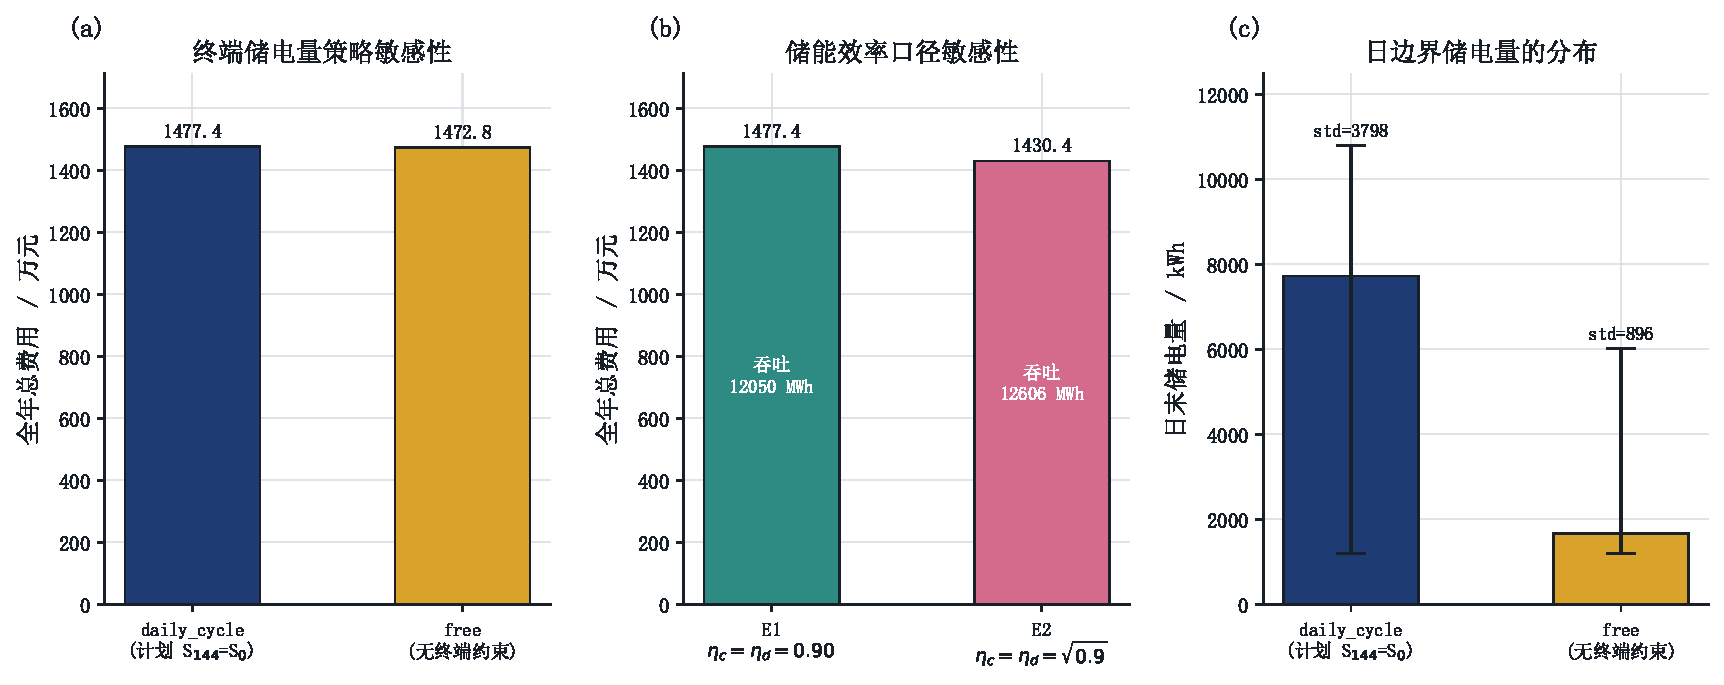
\includegraphics[width=0.98\textwidth]{figures/sensitivity.pdf}
	\caption{终端策略与储能效率口径敏感性}
	\label{fig:sensitivity}
\end{figure}

\subsubsection{储能效率口径}
\label{sec:efficiency}

题目只写“充放电效率为 $90\%$”，存在两种解释：其一，充电效率与放电效率各为 $0.9$（往返效率 $0.81$）；其二，往返总效率为 $0.9$（充放电效率各为 $\sqrt{0.9}\approx0.9487$）。前者是更保守也更为工程界常用的口径，本文主模型采用前者。作为对照，两种口径下的结果列于表~\ref{tab:efficiency}。

\begin{table}[htbp]
	\caption{储能效率口径敏感性}
	\label{tab:efficiency}
	\centering
	\zihao{-5}
	\begin{tabular}{l r r r}
		\toprule
		效率口径 & 全年总费用/元 & 储能吞吐量/kWh & 紧急购电量/kWh \\
		\midrule
		口径 A：$\eta_c=\eta_d=0.90$（往返 $0.81$） & \SensEffEOneCost & \SensEffEOneThroughput & \SensEffEOneEm \\
		口径 B：$\eta_c=\eta_d=\sqrt{0.9}$（往返 $0.90$） & \SensEffETwoCost & \SensEffETwoThroughput & \SensEffETwoEm \\
		\bottomrule
	\end{tabular}
\end{table}

采用往返效率 $0.90$ 时费用更低，因为储能损耗更小、可用于峰谷套利的电量更多。两种口径的结论方向完全一致，说明本文的策略结论不依赖于效率口径的具体解释。

\subsubsection{其他误差来源}

主要误差来源包括三方面：光伏与负载点预测误差、小时预报到 $10$ min 的降尺度误差，以及实际市场价格发布时间的不确定性。前两者已通过历史窗口上的费用代理在线选择、实时反馈和节点消融量化；第三项不改变题面“附件 4 直用”的主答案，因果价格扩展仅用于说明部署时可能的机会成本。这些误差不破坏数值结果的内部一致性，但限制模型直接外推到真实长期运行的精度。
